\section{Kleines Physiker--Überlebens--ABC}


\begin{description}
    \item[Amt für Ausbildungsförderung:] Hier kannst du BAFöG-Formulare
abholen und in ausgefüllter Form wieder abgeben.

    \item[Assistent:] Die
netten (seltener auch nicht netten) Menschen, die in den Praktika
eure Praktikumsprotokolle durchsehen und dann mit der Aufschrift
"`ok"' zurückgeben (oder auch nicht).

    \item[AStA:]Allgemeiner Studierenden Ausschuss.
      Vom \textbf{Stu}dierenden\textbf{pa}rlament gewählt, sozusagen die Regierung desselben.
      Im StuPa tummeln sich die Nachwuchspolitiker
      (Grüne Hochschulgruppe, Juso-Hochschulgruppe, Giraffen - Unabhängige Fachbereichsgruppen,
      RCDS - Ring Christlich-Demokratischer Studenten, Schildkröten, LHG - Liberale Hochschulgruppe,
      attac/independent students, Die Linke.SDS, Pinguine, LiLi - Wahlbündnis Linke Liste,
      DL - Demokratische Linke Liste, FDH - Fachschafteninitiative Demokratische Hochschule)
      und investieren jedes Jahr 500.000 \euro{} für die Studierenden.

    \item[Auslandsstudium:]Wer Interesse an einem Auslandsstudium hat, kann sich bei der Studienberatung
      und beim DAAD informieren.
      Mehr Informationen dazu auch im Kapitel Auslandsstudium (Seite \pageref{sec:Ausland}).

    \item[Ausschüsse:]Der \textbf{F}ach\textbf{b}ereichs\textbf{r}at setzt
verschiedene Ausschüsse ein: So die QSL-Kommision, Prüfungsausschüsse für die einzelnen Studiengänge
und den Studienausschuss.
In allen Ausschüssen sitzen Studierende, die versuchen, die Interessen ihrer Kommiliton(in)en zu
vertreten.

    \item[Bachelor:]Unterste Physikerweihe und seit neuestem auch
berufsqualifizierend. Wird nach sechs Semestern gemacht.

\begin{figure}[!h]
\begin{center}
  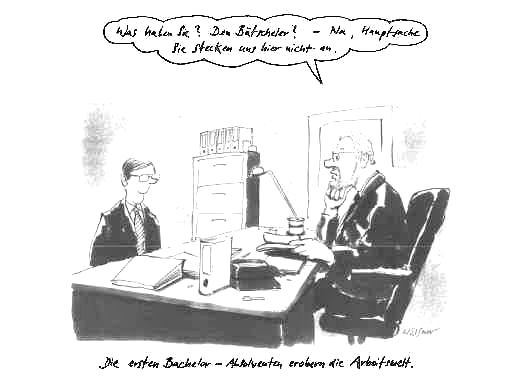
\includegraphics[width=.8\textwidth]{bilder/bachelor.jpg}
\end{center}
\end{figure}

    \item[Bafög:]Bundes-Ausbildungs-Förderungsgesetz.
      Möglichkeit für Studierende, deren Eltern nicht allzuviel verdienen, ein paar Euro
Unterstützung zum Studieren zu bekommen.
Wer meint, dafür in Frage zu kommen, sollte auf jeden Fall einen Antrag beim Amt für
Ausbildungsförderung im Sozialzentrum stellen.
Verlieren kann man nicht viel, nur gewinnen\ldots oder man kriegt nix.

\item[Café Physik:] Eine gute Alternative zur Mensa.
  Mit hübschem Ausblick über die Experimentierhalle.

\item[Campi:] Standorte der Uni.
  Offiziell haben wir momentan 4 + einen Sportcampus.

   \item[Credit Points:] Die Leistungseinheit der neusten Ideen der Bildungsminister:
     Ein Credit Point (CP) stellt angeblich 30 Stunden Arbeitsaufwand für den durchschnittlichen Studierenden dar.
Dieser durchschnittliche Studierende ist allerdings Russe, hat eine Uhr,
auf der zwischen zwei Sonnenaufgängen nur vier Stunden vergehen und nimmt regelmäßig Speed.
In einem Semester solltet ihr etwa 30 CPs sammeln, für den Bachelor müsst ihr 180, für den
Master weitere 120 CPs nachweisen.

    \item[c.t:] "`Cum tempore"': die Veranstaltung beginnt erst nach der "`akademischen`` Viertelstunde.

    \item[Dekan:] Professor, der vom Fachbereichsrat gewählt wird, um ihn nach außen zu vertreten.
      Im Moment ist Prof.Philpsen Dekan des FB13.

    \item[Dekanat:]Verwaltung des Fachbereichs.
      Dem Dekan unterstellt.
      Direkt um die Ecke bei der Fachschaft.

    \item[Didaktik:] Mancher hat sie drauf und mancher halt nicht.
      Auch die Kurzform für das Institut Didaktik der Physik.

    \item[Diplom:] Der Abschluss des Diplomstudiengangs (ist für euch aber sowieso relativ
uninteressant, weil ihr auf BaMa studiert).

    \item[Doppelstudium:]Theoretisch ist es möglich, neben Physik noch ein anderes Fach
(z.B. Mathe oder Philosophie) zu studieren -- L3-ler haben immer
zwei Fächer, allerdings nicht im gleichen Umfang wie Diplom,
Magister oder BaMastudierende. Bei einem Doppelstudiengang sind zeitliche
Kollisionen unvermeidlich und mehr Arbeit ist es natürlich auch.
Dennoch kann man es versuchen; man kann das zweite Fach ja
fallenlassen.

    \item[Dr.h.c:] Doktortitel ehrenhalber (so was wie Helmut
Kohl mal hatte). Um einen Doktortitel führen zu dürfen, muss man
was leisten. Das ist normalerweise eine eigenständige
Forschungsarbeit in der Form der Doktorarbeit. Wenn ein Forscher
(in der Regel ein Prof) für die Wissenschaft in einem Gebiet
herausragendes geleistet hat, kann es passieren, dass eine
Universität diesem Forscher einen Ehrendoktortitel verleiht, mit
dem sich der Ausgezeichnete zusätzlich schmücken darf. Passiert
dies einem Forscher mehrmals (multus, z.B. dem alten Greiner aus der Theorie), darf er sich Prof
Dr.Dr.h.c.mult nennen.

\item[Erstis:] Ihr... und alle anderen, die sich auch noch in höheren Semestern so fühlen.

    \item[Fachschaft:]Die netten Leute, die für
euch diese Handbroschüre und diese Einführungsveranstaltung gemacht
haben. Laut HHG (Hessisches Hochschulgesetz) bilden eigentlich
alle Studierende des Fachbereichs die Fachschaft. Umgangssprachlich
bezeichnet man aber mit "`Fachschaft`` die Gruppe der Studierenden, die
sich für die Interessen der Studierenden am Fachbereich einsetzt. In der
Fachschaft kann man Physikstudierende aus allen Semestern
kennenlernen, die einem auch mal Tipps fürs eigene Studium geben
können. Die Fachschaft sucht ständig neue Leute, also schaut
einfach einmal bei einem Fachschaftstreffen vorbei.

    \item[Fachschaftsrat:]Die Studierenden eines Fachbereiches wählen im
Wintersemester u.a. den Fachbereichsrat. Die gewählten
Studierendenvertreter (und nur die) dürfen offiziell im Namen der
Fachschaft sprechen und Geld ausgeben. In anderen Fachbereichen
läuft das so: Da kandidieren von den hochschulpolitischen
Gruppen der Parteien Vertreter auf eigenen Listen und der
Fachbereichsrat besteht am Ende z.B. 2 Leuten von den Grünen,1
Juso und 2 vom RCDS. Diese liegen sich dann ständig in den Haaren,
weil sie alle nur Parteipolitik machen. Zum Glück sind wir so
wenige und man ist sich einig.

    \item[Fachbereich:]Der Fachbereich (FB)
ist eine nach fachlichen Gesichtspunkten eingegrenzte
Organisationseinheit der Uni. Früher hieß so etwas Fakultät. Es
gibt an der Uni Frankfurt insgesammt 16 FB. Interessant sind für
euch aber hauptsächlich nur FB11 Geowissenschaften, FB12
Mathematik und Informatik, FB13 (der tollste FB überhaupt), FB14
Chemie und FB15 Biologie.

    \item[Fachsbereichsrat:]Trifft sich regelmäßig und bespricht
alles, was den Fachbereich irgendwie angeht, besteht aus Profs,
Studierenden, wissenschaftlichen Mitarbeitern und
administrativ-technischem Personal.

    \item[Freizeit:] Was ist denn das?

\item[Goethe--Card:] Bekommt ihr, wenn ihr sie nicht schon habt, im StudierendenServiceCenter in Bockenheim.
Sie ist gleichzeitig Studierendenausweis, RMV-Ticket, Bibliotheksausweis, Eintrittskarte für den Palmengarten und ihr könnt damit in der Mensa bezahlen.

\item[Greiner, Walter:]
Ist der berühmteste Professor der letzten Zeit aus Frankfurt und
hat zu Alledem noch die roten "`Physikbibeln`` geschrieben.

    \item[Harri Deutsch:] Verlag aus Frankfurt, der auch einige Physikb\"ucher im Programm hat.

    \item[HiWis:] Hilfswissenschaftler, Sklaven der Professoren.

    \item[HRZ:]Hochschulrechenzentrum, das sind die Leute, die euch nen Account
geben und mit denen ihr euch rumschlagt (oder sie mit euch), wenn
der Computer mal spinnt.

    \item[Institute:]Da gibt es zum einen das
Physikalische Institut, das Institut für Theoretische Physik, die
Angewandte Physik, Kernphysik, Biophysik sowie das Institut für Didaktik der Physik.

    \item[Internet:]Beliebtes
Mittel, um beispielsweise Protokolle auszutauschen.\\
www.fachschaft.physik.uni-frankfurt.de ist auch dafür eine
tolle Adresse im Netz.

    \item[Klausur:] In Physik werden euch mit dem BaMa-Studiengang
wahrscheinlich des öfteren mal Klausuren begegnen.
Normalerweise benötigt ihr nur 50\% der erreichbaren Punkte um zu bestehen und
wenn das nicht klappt, könnt ihr es nochmal versuchen\ldots oder Pech
gehabt.

    \item[Klopfen:] Komische Tradition nach der Vorlesung. Wird
wahrscheinlich gemacht, um die Leute zu wecken.

    \item[Kolloquium:]Eigentlich mündliche Prüfung bei Professor oder Assistent.
    Dann gibt es noch das physikalische Kolloquium, eine Veranstaltung mittwochsabends.
Da reden dann auswärtige Wissenschaftler über ihre aktuelle Forschung.
Man versteht oft rein gar nichts, es ist aber trotzdem empfehlenswert, hinzugehen!

    \item[Kommilitonen:] Eure Mitstudierenden.

\item[Linguisten:] Haben was mit Sprache und Verständnis zu tun, interessieren uns also nicht.

\item[Master:] Hört sich an wie bei Konfuzius, ist es auch fast.
Wenn ihr den habt, seid ihr schon fast weise.

    \item[Mathevorlesung:]Dienstag und Donnerstag von 8-10.
 Meist der Graus aller neuen Physiker, doch es
ist durchaus zu schaffen und eigentlich nicht uninteressant.
Blüht euch aber erst im Wintersemester.

    \item[Mensa:]Je mehr der Speiseplan verspricht, desto mehr Vorsicht!

\begin{figure}[!h]
 \begin{center}
  
\includegraphics[width=\textwidth]{bilder/yes.jpg}
 \end{center}
\end{figure}

\item[Modul:]
Wie ein Puzzleteil\ldots Ihr müsst viele sammeln und richtig zusammen stecken, dann
kommt ein Abschluss dabei raus.

    \item[Nebenfach:]Notwendiges Übel oder Spaß.
    Das liegt meist an der Wahl des Nebenfaches.

    \item[Physikerinnen:]Aufstrebende Gattung, die diese Männerdomäne immer mehr überollt.
    Ihr dürft sie auch ansprechen ;)

    \item[Praktikum:] Eigentlich:"`Physikalisches Anfängerpraktikum Teil I und Teil II``.
Spielstunde am Nachmittag, in der es um Mechanik/Thermodynamik/Optik (Teil I) bzw.
Elektrodynamik (Teil II) geht. Zusätzlich zum Experimentieren
wollen Protokolle geschrieben werden (Übel).

    \item[Präsident:]Selbstklärend, oder?

    \item[Prof. emeritus:]Professor, der eigentlich schon
im Ruhestand ist, aber trotzdem noch im Institut rumgurkt.

    \item[Promotion:] Erhebung auf ein höheres Level.
    Wer promoviert hat, darf sich ein Dr. vor den Namen klatschen.

\item[Psychologische Beratung:] Braucht ihr, nachdem ihr das Studierendensekreteriat verlassen habt.

    \item[Regelstudienzeit:]Für euch sechs Semester (bis zum Bachelor)\ldots

    \item[s.t.:]"`Sine tempore``: bist du
nicht zur gegebenen Zeit da, brauchst du ne gute Ausrede.

    \item[Scheine:]Genau wie mit dem Geld: "`sammeln und drauf aufpassen``.
    Für eure Bachelorprüfung braucht ihr diverse Modulzertifikate.
In der Physik musst du für die Scheine regelmäßig vorrechnen und Aufgaben
abgeben.

    \item[Semesterferien:]\ldots gibt's nicht.
    Nur eine vorlesungsfreie Zeit.
In dieser Zeit muss man für die Klausuren (ja, die finden alle in den "`Ferien`` statt)
lernen und kann Blockpraktika machen oder einfach nur faulenzen. In höheren Semestern
wird man auch in dieser Zeit an der Uni arbeiten, z.B. an der
Abschlussarbeit.

    \item[Semesterticket:]Eine der praktischsten Erfindungen
seit geschnittenem Brot! Eure Fahrkarte für das gesammte RMV-Netz,
nie wieder wird man so billig die öffentlichen Verkehrsmittel
nutzen können!!

    \item[Seminar:]Veranstaltung, in der
Vorträge gehalten werden. Gibt es einen Schein für das Seminar,
muss man im Normalfall auch selbst einen halten.

    \item[Senat:]Ist die zentrale Vertretung aller Statusgruppen der Universität.

    \item[Sozialzentrum:]Das Gebäude, in dem sich u.a. Studierendensekretariat, Mensa und
BaFöG-Amt (genauer: Amt für Ausbildungsförderung) befinden.

    \item[Sport:]Empfehlenswert, gerade das Zentrum für Hochschulsport (ZfH) bietet coole Kurse an!

    \item[Stipendien:]Wer gute Schul-/Studienleistungen vorzuweisen hat,
sollte sich um ein Stipendium bemühen.
Selbst vorschlagen kann man sich mitlerweile bei allen zwölf staatlichen Stiftungen.
Das sind die parteinahen (Konrad-Adenauer-Stiftung
(CDU-nah), Friedrich-Ebert-Stiftung (SPD-nah),
Friedrich-Nauman-Stiftung (FDP-nah), Heinrich-Böll-Stiftung
(Grüne-nah) und Rosa-Luxemburg-Stiftung (Linke-nah)),
die kirchlichen Stiftungen (Cusanuswerk (katholisch), Studienwerk Villigst (evangelisch)
und das Ernst Ludwig Ehrlich Studienwerk (jüdisch)),
die Stiftung der Deutschen Wirtschaft und die Studienstiftung des Deutschen Volkes.
Neben den Studienleistungen spielt bei allen Stiftungen auch
gesellschaftliches, soziales, politisches und/oder kirchliches
Engagement eine Rolle.
Nähere Informationen zu Stipendien gibt es in der zentralen Studienberatung.
Bewerben lohnt sich auf jeden Fall!!

    \item[Studierendensekretariat:]Unter der Mensa in Bockenheim,
dort kann man sich rückmelden und allerlei Bescheinigungskram
bekommen, vor Allem aber stundenlang anstehen, um mit überaus netten und zuvorkommenden
Menschen zu diskutieren, wenn mal nicht alles so klappt, wie man will.

    \item[Studierendenenwerk:] Die netten Leute, die uns z.B. in der Mensa
mit Essen versorgen.

    \item[Studienberatung:]Machen Prof. Wagner und Prof. Roskos (für Physik),
, Prof. Mäntele (für Biophysik),
    Prof. Engel (für Computational Science) und Frau Korneck und Herr Ritter
    (für Lehramt).
Helfen bei allen Fragen, die beim
Studium so auftauchen können ("`Bin ich denn wahnsinnig?"',
"`Warum tue ich mir denn das alles an?"').
%Beklagen sich manchmal über zu wenig Arbeit.
%Zu finden in Gebäudeteil 4 ganz unten.
%Aber auch wir sind immer f\"ur Fragen offen.

\begin{center}
    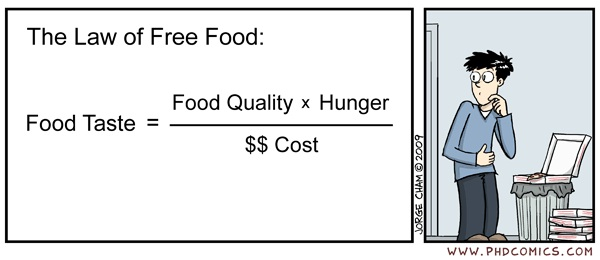
\includegraphics[width=.9\textwidth]{bilder/food.jpg}
\end{center}

\item[Studiengebühren:] Haben wir zum Gl\"uck nicht mehr.
ABER man kann nie wissen.
Also seid achtsam!

\item[Thai:] Imbiss gegen\"uber der Bushaltestelle.
Wen das Mensaessen nicht krank gemacht hat, kann sein Gl\"uck hier versuchen.

 \item[Theoretikum:]Übungen in der Theoretischen Physik, wie Praktikum, nur
theoretisch.

    \item[Tutor:] Das sind Studierende höherer Semester, die eure
Übungsgruppen betreuen und eure Aufgaben korrigieren.
Freuen sich, wenn ihr sie mit Fragen löchert.

    \item[Übungen:]
Zum einen die kleinen, gemeinen Zettel, die ihr wöchentlich bekommt.
Dann gibt es aber auch die Übungsstunde, in denen die Dinger dann besprochen werden.

%    \item[Volkssternwarte:] Oben im physikalischen Verein, Freitags gibts da
%Vorträge und Sterne gucken kann man auch. Der Eingang ist übrigens
%an der Rückseite des alten Physikgebäudes in Bockenheim.

    \item[Wahlen:]Du darfst im Wintersemester wählen.
    Und du sollst es auch, denn die
Demokratie lebt vom Mitmachen und dir ist doch die Demokratie
lieber als die Diktatur, oder etwa nicht? Schliesse dich also der
wählenden Minderheit an\ldots ansonsten wird dem AStA das Geld
gekürzt und die können dann nicht mehr so viel machen, wie z.B.
für euer Semesterticket kämpfen.
Im Einzelnen wählst du
Fachschaftsrat und Fachbereichsrat (Physik-intern) sowie
Studierendenparlament und den Senat (Uni-weit).

    \item[WiWis:]Wirtschaftswissenschaftler.
    Der Fachbereich mit den meisten Studierenden (über 4000).
 Sitzt am Westend.
 Wird von manchen als Erzfeind angesehen, für diese
Bezeichnung eignen sich die Mathematiker aber wesentlich besser.

\item[Zentralmensa:]In Bockenheim.
Seid froh, dass ihr da nicht essen müsst.

%\begin{center}
%    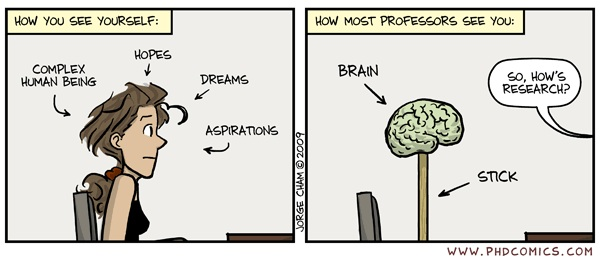
\includegraphics[width=1.00\textwidth]{bilder/ansehen.jpg}
%\end{center}

\end{description}
%
%\begin{figure}[!h]
% \begin{center}
%  \includegraphics[height=\textheight]{bilder/phd.jpg}
% \end{center}
%\end{figure}
